\documentclass[12pt,pdf,hyperref={unicode}]{beamer}
%\usetheme{boxes}
\beamertemplatenavigationsymbolsempty
\setbeamertemplate{footline}[page number]
% Set it for the internal PhD thesis defence to reduce number of slides
%\setbeamersize{text margin left=0.5em, text margin right=0.5em}

\usepackage[utf8]{inputenc}
%\usepackage[english, russian]{babel}
\usepackage{bm}
\usepackage{multirow}
\usepackage{ragged2e}
\usepackage{indentfirst}
\usepackage{multicol}
\usepackage{subfig}
\usepackage{amsmath,amssymb}
\usepackage{enumerate}
\usepackage{mathtools}
\usepackage{comment}
\usepackage[all]{xy}
\usepackage{tikz}
\usetikzlibrary{positioning,arrows}
\tikzstyle{name} = [parameters]
\definecolor{name}{rgb}{0.5,0.5,0.5}

%\usepackage{caption}
%\captionsetup{skip=0pt,belowskip=0pt}

%\newtheorem{theorem}{Theorem}
%\newtheorem{statement}{Statement}
%\newtheorem{definition}{Definition}

% colors
\definecolor{darkgreen}{rgb}{0.0, 0.2, 0.13}
\definecolor{darkcyan}{rgb}{0.0, 0.55, 0.55}
%\AtBeginEnvironment{figure}{\setcounter{subfigure}{0}}
%\captionsetup[subfloat]{labelformat=empty}

%----------------------------------------------------------------------------------------------------------

\title{ Put the title of your thesis \\ here}
%\author{Name Surname}
%\institute[]{}
%\date{2024}

%---------------------------------------------------------------------------------------------------------
\begin{document}

%\begin{frame}
%\titlepage
%\end{frame}
\setcounter{page}{1}%remove here for the title
%----------------------------------------------------------------------------------------------------------
%\section{Please do not use sectioning in the presentations}
\begin{frame}{Banking credit scoring}
\begin{block}{Shakhov Stanislav}
\end{block}
\end{frame}
%----------------------------------------------------------------------------------------------------------
%\section{Please do not use sectioning in the presentations}
\begin{frame}{Banking credit scoring}
It is proposed to improve the existing banking scoring systems by changing the approach to calculating the risk for the client. 

\begin{block}{Goal}
To improve the current risk calculation process, which takes into account only the probability of the customer's default during the specified period. 
\end{block}
\begin{block}{Alternative}
Modelling the customer's credit behavior throughout the entire term and, based on this, predict the risk.
\end{block}
\begin{block}{Choise reasoning} 
\begin{enumerate}[1)]
\item the new solution implies forecasting some events that may occur: the probability of a customer's default and recover, the share of depreciation of his loan, 
\item the risk forecast will take into account a larger number of input parameters.

\end{enumerate}
\end{block}
\end{frame}
%----------------------------------------------------------------------------------------------------------
\begin{frame}{Banking credit scoring}
The dependence of margin on overdue debt and duration 
\begin{columns}
\begin{column}{0.4\textwidth}
\begin{enumerate}[1)]
    \item Margin - the share of the bank's income from the loan amount 
    \item Debt  - normalized overdue loan amount 
    \item Duration - The normalized cumulative amount of a healthy customer balance by year 
\end{enumerate}
\end{column}
\begin{column}{0.6\textwidth}
\begin{figure}
    \centering
    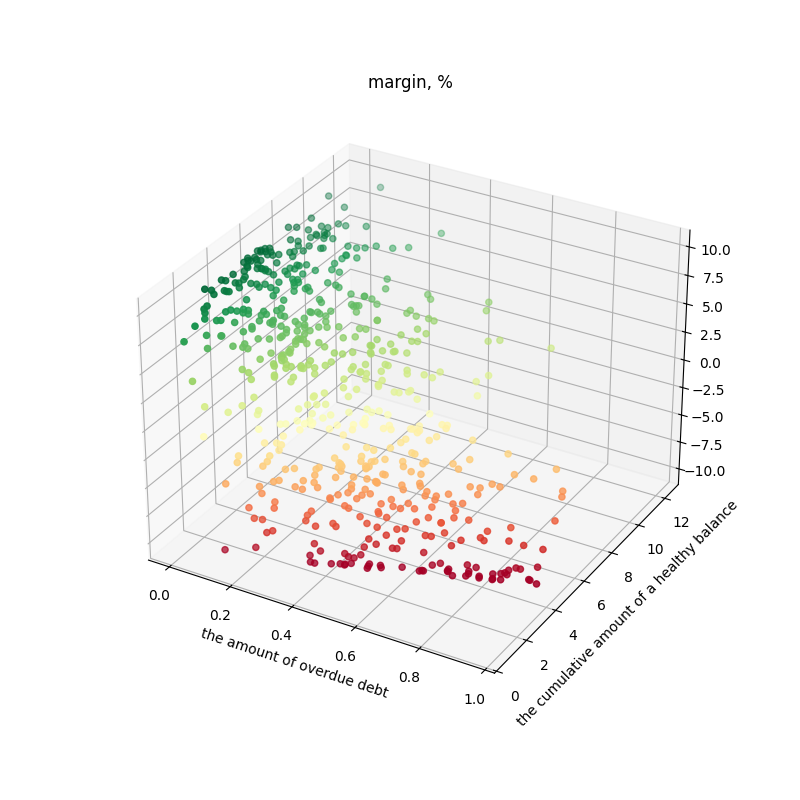
\includegraphics[width=1\linewidth]{margin.png}

\end{figure}
\end{column}
\end{columns}
\bigskip
\end{frame}
\end{document}